\documentclass[french,a4paper,10pt]{article}
% pdflatex compte_rendu.tex -output-directory=out && mv out/compte_rendu.pdf ./

\usepackage[a4paper,hmargin=30mm,vmargin=30mm]{geometry}
\usepackage[T1]{fontenc} % font type
\usepackage[french]{babel} % language
\usepackage{lmodern} % font type
\usepackage[shortlabels]{enumitem}
\usepackage{hyperref}
\usepackage{graphicx}
\usepackage{sectsty}
%\setlength{\parindent}{0pt}



\title{Compte Rendu TP4\\
Détection de contours d'une image\\
avec utilisation du gradient (1er ordre)}
\author{Ivan Lejeune}
\date{\today}


\begin{document}
    \maketitle

    % make table of contents
    \tableofcontents

    \newpage
    \section{Création de la carte de gradient d'une image}\label{sec:1}

    \subsection{Programme}\label{subsec:1.1}

    On commence par créer le programme \texttt{norme\_gradient.cpp} qui en chaque point d'une image calcule les
    gradients horizontaux et verticaux, puis retourne la norme du gradient.
    On crée ensuite une nouvelle image avec les valeurs de la norme du gradient.
    Enfin, on comparera les profils d'une ligne de l'image originale et de l'image de la norme du gradient.

    L'essentiel du code est le suivant : % insert code as image
    \begin{figure}[!htb]
        \centering
        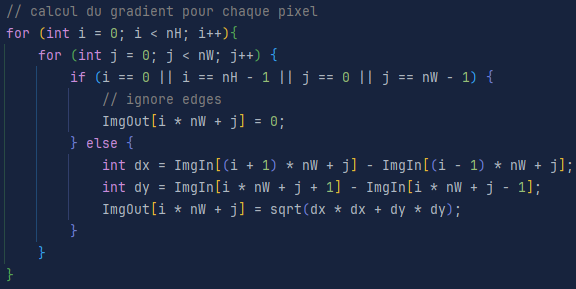
\includegraphics[width=0.7\textwidth]{out/code-norme-gradient}
        \caption{Code de norme\_gradient.cpp}\label{fig:code-norme-gradient}
    \end{figure}

    La transformation de l'image donne : % insert both images
    \begin{figure}[!htb]
        \begin{minipage}{0.48\textwidth}
            \centering
            \fbox{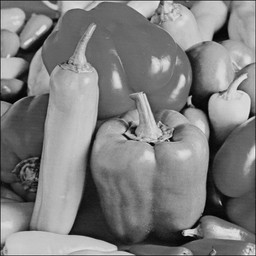
\includegraphics[width=.7\linewidth]{./out/peppers-grey}}
            \caption{Image originale}\label{Fig:peppers-grey}
        \end{minipage}\hfill
        \begin{minipage}{0.48\textwidth}
            \centering
            \fbox{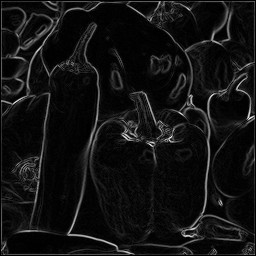
\includegraphics[width=.7\linewidth]{./out/gradient-peppers-grey}}
            \caption{Image de la norme}\label{Fig:gradient-peppers-grey}
        \end{minipage}
    \end{figure}

    On peut voir que les contours de l'image sont bien mis en évidence.

    \newpage
    \subsection{Comparaison des profils}\label{subsec:1.2}

    On compare les profils d'une ligne de l'image originale et de l'image de la norme du gradient.
    On peut voir que les contours sont bien mis en évidence sur l'image de la norme du gradient.

    La différence entre les deux profils est bien visible sur la colonne 80 : % insert profiles
    \begin{figure}[!htb]
        \centering
        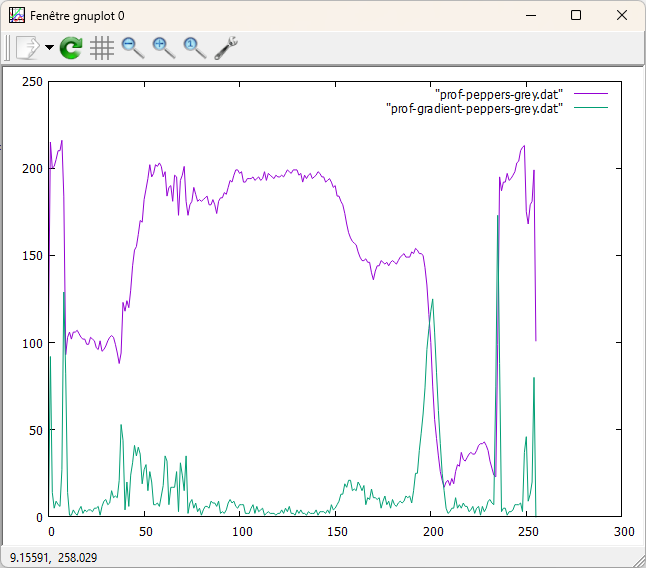
\includegraphics[width=0.7\textwidth]{out/prof-peppers-grey-gradient}
        \caption{Comparaison des profils}\label{fig:profiles}
    \end{figure}

    \newpage
    \section{Extraction des maxima locaux par seuillage}\label{sec:2}

    On va extraire des maxima locaux de l'image de la norme du gradient par seuillage.
    On crée un programme \texttt{maxima\_locaux.cpp} qui prend en entrée une image de la norme du gradient et un seuil.
    Le programme retourne une image binaire avec les maxima locaux.

    L'essentiel du code est le suivant : % insert code as image
    \begin{figure}[!htb]
        \centering
        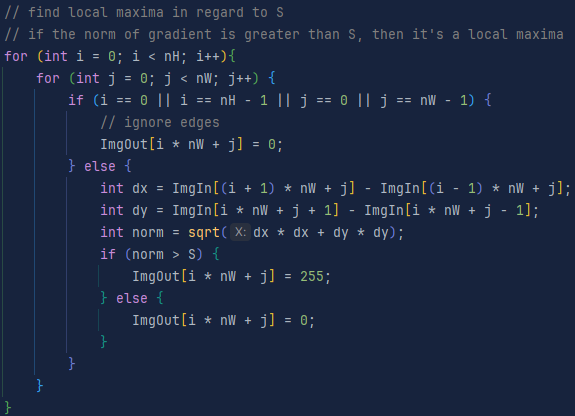
\includegraphics[width=0.7\textwidth]{out/code-maxima-locaux}
        \caption{Code de maxima\_locaux.cpp}\label{fig:code-maxima-locaux}
    \end{figure}

    On applique le programme sur l'image de la norme du gradient avec 3 seuils différents, ici 80, 60 et 30 : % insert images

    \begin{figure}[!htb]
        \begin{minipage}{0.3\textwidth}
            \centering
            \fbox{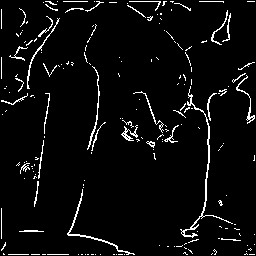
\includegraphics[width=.7\linewidth]{./out/maxima-80-peppers-grey}}
            \caption{Image avec un seuil de 80}\label{Fig:maxima-80-peppers-grey}
        \end{minipage}\hfill
        \begin{minipage}{0.3\textwidth}
            \centering
            \fbox{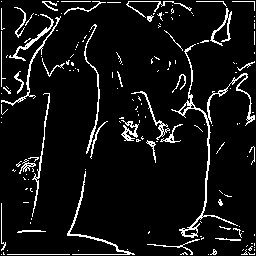
\includegraphics[width=.7\linewidth]{./out/maxima-60-peppers-grey}}
            \caption{Image avec un seuil de 60}\label{Fig:maxima-60-peppers-grey}
        \end{minipage}\hfill
        \begin{minipage}{0.3\textwidth}
            \centering
            \fbox{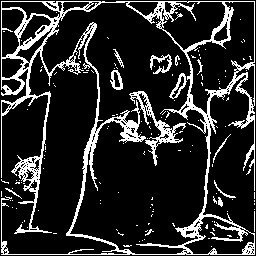
\includegraphics[width=.7\linewidth]{./out/maxima-30-peppers-grey}}
            \caption{Image avec un seuil de 30}\label{Fig:maxima-30-peppers-grey}
        \end{minipage}
    \end{figure}

    On peut voir que plus le seuil est bas, plus les maxima locaux sont nombreux, et donc plus de contours sont
    détectés.

    \newpage
    \section{Seuillage par hystérésis des maxima locaux}\label{sec:3}

    On va maintenant appliquer un seuillage par hystérésis sur l'image de la norme du gradient.
    On crée un programme \texttt{hysteresis.cpp} qui prend en entrée une image de la norme du gradient et deux seuils.
    Le programme retourne une image binaire avec les contours détectés.

    L'essentiel du code est le suivant : % insert code as 2 images
    \begin{figure}[!htb]
        \begin{minipage}{0.48\textwidth}
            \centering
            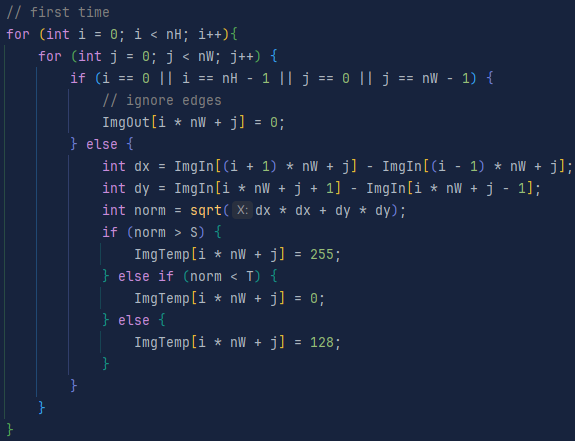
\includegraphics[width=0.7\textwidth]{out/code-hysteresis1}
            \caption{Code de hysteresis.cpp (1/2)}\label{fig:code-hysteresis1}
        \end{minipage}\hfill
        \begin{minipage}{0.48\textwidth}
            \centering
            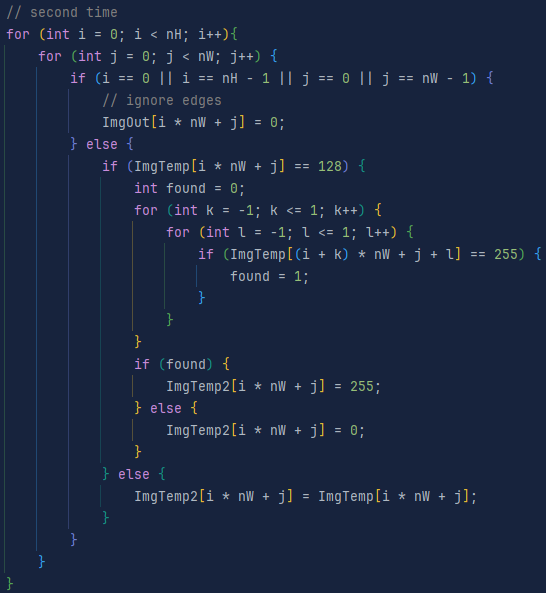
\includegraphics[width=0.7\textwidth]{out/code-hysteresis2}
            \caption{Code de hysteresis.cpp (2/2)}\label{fig:code-hysteresis2}
        \end{minipage}
    \end{figure}

    On applique le programme sur l'image de la norme du gradient avec trois paires de seuils différents,
    ici (80, 60), (60, 30) et (30, 10) : % insert images
    \begin{figure}[!htb]
        \begin{minipage}{0.3\textwidth}
            \centering
            \fbox{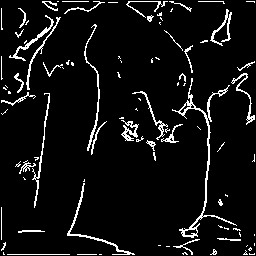
\includegraphics[width=.7\linewidth]{./out/hysteresis-80-60-peppers-grey}}
            \caption{Image avec des seuils de 80 et 60}\label{Fig:hysteresis-80-60-peppers-grey}
        \end{minipage}\hfill
        \begin{minipage}{0.3\textwidth}
            \centering
            \fbox{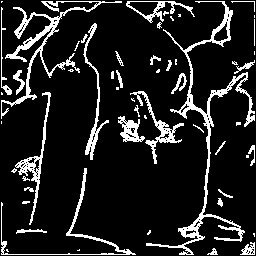
\includegraphics[width=.7\linewidth]{./out/hysteresis-60-30-peppers-grey}}
            \caption{Image avec des seuils de 60 et 30}\label{Fig:hysteresis-60-30-peppers-grey}
        \end{minipage}\hfill
        \begin{minipage}{0.3\textwidth}
            \centering
            \fbox{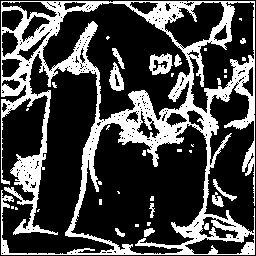
\includegraphics[width=.7\linewidth]{./out/hysteresis-30-10-peppers-grey}}
            \caption{Image avec des seuils de 30 et 10}\label{Fig:hysteresis-30-10-peppers-grey}
        \end{minipage}
    \end{figure}

    On peut voir que plus les seuils sont bas, plus de contours sont détectés.

    \newpage
    \section{Prétraitement par filtrage}\label{sec:4}

    On recommence les étapes précédentes avec une image prétraitée par filtrage.

    \subsection{Filtre moyenneur}\label{subsec:4.1}

    On crée un programme \texttt{filtre\_moyenneur.cpp} qui prend en entrée une image et un masque de filtrage.
    Le programme retourne une image filtrée.

    L'essentiel du code est le suivant : % insert code as image
    \begin{figure}[!htb]
        \centering
        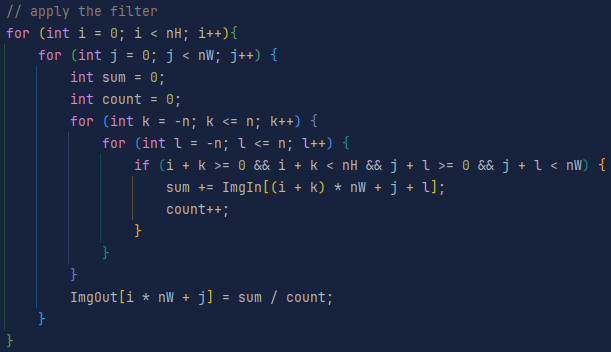
\includegraphics[width=0.7\textwidth]{out/code-filtre-moyenneur}
        \caption{Code de filtre\_moyenneur.cpp}\label{fig:code-filtre-moyenneur}
    \end{figure}

    On applique le programme sur l'image originale avec un masque de 3x3 : % insert images
    \begin{figure}[!htb]
        \begin{minipage}{0.48\textwidth}
            \centering
            \fbox{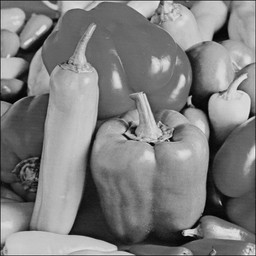
\includegraphics[width=.7\linewidth]{./out/peppers-grey}}
            \caption{Image originale}\label{Fig:peppers-grey-1}
        \end{minipage}\hfill
        \begin{minipage}{0.48\textwidth}
            \centering
            \fbox{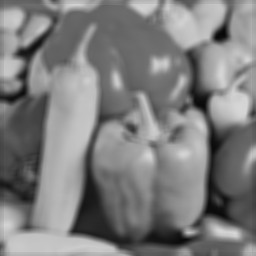
\includegraphics[width=.7\linewidth]{./out/filtre-moyenneur-peppers-grey}}
            \caption{Image filtrée}\label{Fig:filtre-moyenneur-peppers-grey}
        \end{minipage}
    \end{figure}

    \newpage
    \subsection{Filtre gaussien}\label{subsec:4.2}

    On crée un programme \texttt{filtre\_gaussien.cpp} qui prend en entrée une image et un masque de filtrage.
    Le programme retourne une image filtrée.

    L'essentiel du code est le suivant : % insert code as image
    \begin{figure}[!htb]
        \centering
        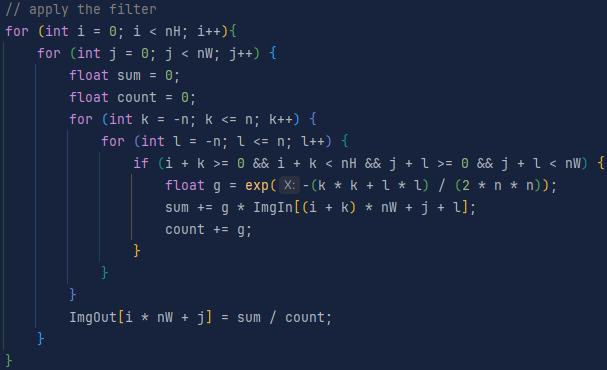
\includegraphics[width=0.7\textwidth]{out/code-filtre-gaussien}
        \caption{Code de filtre\_gaussien.cpp}\label{fig:code-filtre-gaussien}
    \end{figure}

    On applique le programme sur l'image originale avec un masque de 3x3 : % insert images
    \begin{figure}[!htb]
        \begin{minipage}{0.48\textwidth}
            \centering
            \fbox{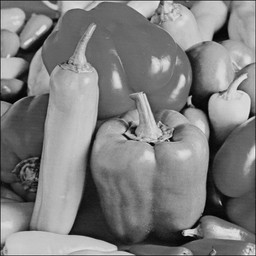
\includegraphics[width=.7\linewidth]{./out/peppers-grey}}
            \caption{Image originale}\label{Fig:peppers-grey-2}
        \end{minipage}\hfill
        \begin{minipage}{0.48\textwidth}
            \centering
            \fbox{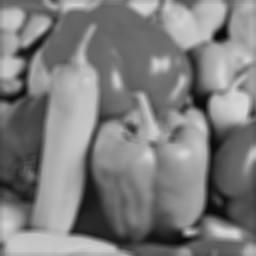
\includegraphics[width=.7\linewidth]{./out/filtre-gaussien-peppers-grey}}
            \caption{Image filtrée}\label{Fig:filtre-gaussien-peppers-grey}
        \end{minipage}
    \end{figure}

    \newpage
    \subsection{Résultats}\label{subsec:4.3}

    On recommence les étapes précédentes avec les images filtrées par les deux filtres.

    On applique le programme \texttt{norme\_gradient.cpp} sur les images filtrées par les deux filtres : % insert images

    \begin{figure}[!htb]
        \begin{minipage}{0.48\textwidth}
            \centering
            \fbox{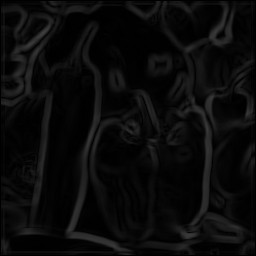
\includegraphics[width=.7\linewidth]{./out/gradient-filtre-moyenneur-peppers-grey}}
            \caption{Image de la norme avec filtre moyenneur}\label{Fig:gradient-filtre-moyenneur-peppers-grey}
        \end{minipage}\hfill
        \begin{minipage}{0.48\textwidth}
            \centering
            \fbox{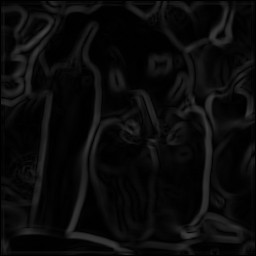
\includegraphics[width=.7\linewidth]{./out/gradient-filtre-gaussien-peppers-grey}}
            \caption{Image de la norme avec filtre gaussien}\label{Fig:gradient-filtre-gaussien-peppers-grey}
        \end{minipage}
    \end{figure}

    On applique le programme \texttt{maxima\_locaux.cpp} sur les images de la norme avec les deux filtres : % insert images

    \begin{figure}[!htb]
        \begin{minipage}{0.48\textwidth}
            \centering
            \fbox{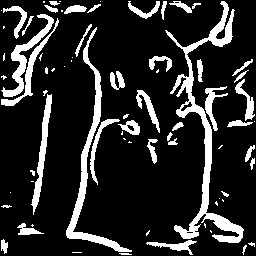
\includegraphics[width=.7\linewidth]{./out/maxima-20-filtre-moyenneur-peppers-grey}}
            \caption{Image avec filtre moyenneur et seuil de 20}\label{Fig:maxima-20-gradient-filtre-moyenneur-peppers-grey}
        \end{minipage}\hfill
        \begin{minipage}{0.48\textwidth}
            \centering
            \fbox{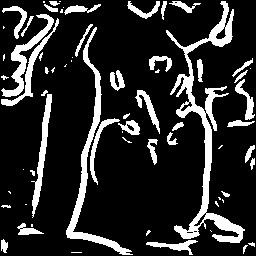
\includegraphics[width=.7\linewidth]{./out/maxima-20-filtre-gaussien-peppers-grey}}
            \caption{Image avec filtre gaussien et seuil de 20}\label{Fig:maxima-20-gradient-filtre-gaussien-peppers-grey}
        \end{minipage}
    \end{figure}

    On applique le programme \texttt{hysteresis.cpp} sur les images de la norme avec les deux filtres : % insert images

    \begin{figure}[!htb]
        \begin{minipage}{0.48\textwidth}
            \centering
            \fbox{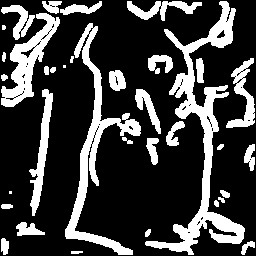
\includegraphics[width=.7\linewidth]{./out/hysteresis-20-10-filtre-moyenneur-peppers-grey}}
            \caption{Image avec filtre moyenneur et seuils de 20 et 10}\label{Fig:hysteresis-20-10-gradient-filtre-moyenneur-peppers-grey}
        \end{minipage}\hfill
        \begin{minipage}{0.48\textwidth}
            \centering
            \fbox{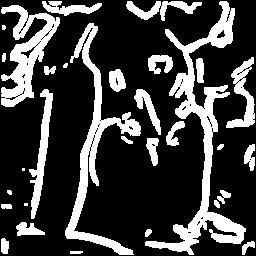
\includegraphics[width=.7\linewidth]{./out/hysteresis-20-10-filtre-gaussien-peppers-grey}}
            \caption{Image avec filtre gaussien et seuils de 20 et 10}\label{Fig:hysteresis-20-10-gradient-filtre-gaussien-peppers-grey}
        \end{minipage}
    \end{figure}

    \newpage
    \section{Conclusion}\label{sec:5}

    On a vu que les contours d'une image peuvent être détectés avec le gradient de l'image.
    On a aussi vu que le filtrage de l'image peut améliorer la détection des contours.
    On a donc pu comparer les résultats de la détection de contours avec et sans filtrage.

\end{document}